\chapter{Systemkonzeption}


\section{�berblick}

 - Fehler bei der Darstellung -> Fehlerwert ausnutzen\\
 - Visueller/Progressiver Ansatz (outputsensitiv)\\
 - Problem bei Visuellen Ansatz: Mann muss das was man sieht einordnen k�nnen


\section{Datenstruktur}


\section{Aufbau}
\begin{figure}[position=h]
  \centering
  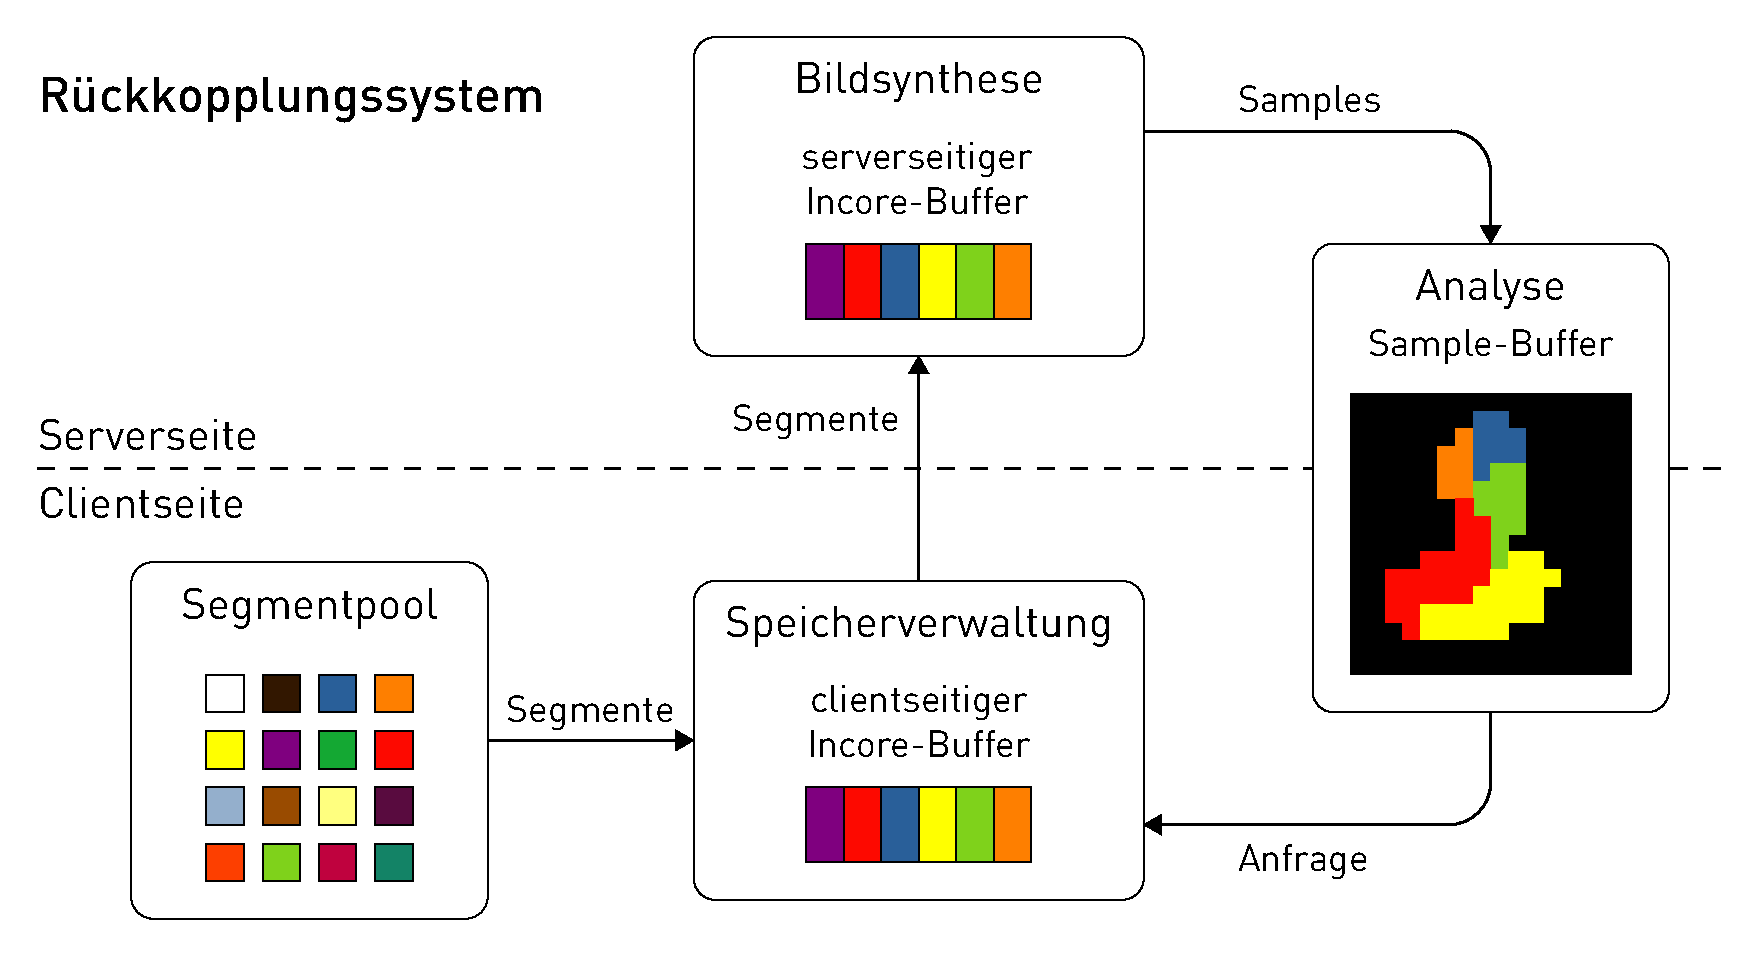
\includegraphics[width=0.85\textwidth]{figures/out-of-core_setup.pdf}
  \caption{Schematischer Aufbau des Out-Of-Core-Systems\label{out-of-core_setup1}}
\end{figure}

\section{Out-of-Core Management}


\section{Real Time Rendering von SVO}
